\documentclass[conference]{IEEEtran}
\IEEEoverridecommandlockouts
\usepackage{cite}
\usepackage{amsmath,amssymb,amsfonts}
\usepackage{algorithmic}
\usepackage{graphicx}
\usepackage{textcomp}
\usepackage{xcolor}
\usepackage{subcaption}
\usepackage{booktabs}
\def\BibTeX{{\rm B\kern-.05em{\sc i\kern-.025em b}\kern-.08em
    T\kern-.1667em\lower.7ex\hbox{E}\kern-.125emX}}
\begin{document}

\title{Comparison of Kalman Filter, Extended Kalman Filter,\\
       and Particle Filter for Mobile Robot Localization}

\author{\IEEEauthorblockN{Viktoriia Ovdiienko}\\
\IEEEauthorblockA{FH Technikum Wien, Vienna, Austria}
}

\maketitle

%%%%%%%%%%%%%%%%%%%%%%%%%%%%%%%%%%%%%%%%%%%%%%%%%%%%%%%%%%%%%%%%%%
\begin{abstract}
Accurate localization is a fundamental requirement for autonomous mobile robots
operating in partially observable environments.
This paper compares three probabilistic state estimation algorithms ---
the Kalman Filter (KF), the Extended Kalman Filter (EKF), and the Particle Filter (PF) ---
for a unicycle robot that uses noisy IMU measurements and known landmarks.
All three filters are implemented as ROS\,2 nodes in C++ and evaluated on an
identical S-shaped slalom trajectory that travels from the lower-left to the
upper-right of the map while weaving between nine obstacle blocks.
Performance is measured by root-mean-square error (RMSE) against ground truth,
heading error, per-step runtime, and the evolution of estimated uncertainty.
Beyond the baseline comparison, the three mandatory experiments are carried out:
process-noise ($Q$) variation, measurement-noise ($R$) variation, and
time-delayed measurements (0, 100 and 500\,ms).
On the asymmetric slalom the PF achieves the lowest position RMSE
($0.011$\,m), the EKF is intermediate ($0.102$\,m), and the KF is the least
accurate ($0.312$\,m), confirming the theoretical ordering.
RMSE increases monotonically with measurement delay for all filters, the PF
being most sensitive, while the $Q$ and $R$ sweeps both exhibit U-shaped optima
that quantify the model-confidence versus sensor-trust trade-off.
\end{abstract}

%%%%%%%%%%%%%%%%%%%%%%%%%%%%%%%%%%%%%%%%%%%%%%%%%%%%%%%%%%%%%%%%%%
\section{Introduction}

Mobile robot localization --- determining a robot's pose from noisy sensor data ---
is a core problem in probabilistic robotics \cite{Thrun2005Probabilistic}.
Without reliable pose estimates, higher-level tasks such as path planning and
object manipulation cannot be performed safely.

A robot equipped only with an inertial measurement unit (IMU) accumulates
heading errors that grow without bound over time, a phenomenon known as
\emph{odometry drift}.
Occasional observations of a known landmark provide absolute corrections that
bound this drift, but the resulting nonlinear, non-Gaussian estimation problem
requires careful algorithmic treatment.

Three classes of filters are widely used: the linear KF, which is optimal for
Gaussian linear systems \cite{Kalman1960New}; the EKF, which extends the KF
to mildly nonlinear systems via first-order Taylor linearisation
\cite{Bar-Shalom2001Estimation}; and the PF (Monte Carlo Localization),
which represents the belief distribution with a set of weighted samples and
can handle arbitrary nonlinearity and multi-modality \cite{Dellaert1999Monte}.

The \textbf{contribution} of this paper is a systematic empirical comparison of
all three filters on identical data from a ROS\,2 simulation, using an
obstacle-avoiding S-slalom trajectory rather than a symmetric circle.
We quantify the accuracy versus computational-cost trade-off, analyse the
process- and measurement-noise sensitivity, and examine how artificial
measurement delays affect each filter.
We additionally document the engineering problems encountered during
development and how they were resolved.

The paper is structured as follows.
Section~\ref{sec:soa} reviews related work.
Section~\ref{sec:methods} describes the system model, the trajectory, the filter
implementations and the practical challenges.
Section~\ref{sec:results} presents and discusses the results.
Section~\ref{sec:summary} summarises findings and outlines future work.

%%%%%%%%%%%%%%%%%%%%%%%%%%%%%%%%%%%%%%%%%%%%%%%%%%%%%%%%%%%%%%%%%%
\section{State of the Art}
\label{sec:soa}

The Kalman filter, introduced by Kalman in 1960, provides the closed-form
minimum-variance estimate for linear systems with Gaussian noise
\cite{Kalman1960New}.
For robot localization, however, the motion and sensor models are inherently
nonlinear, motivating extensions.

Smith and Cheeseman \cite{Smith1986Estimating} introduced the concept of stochastic
maps using EKF to jointly estimate robot pose and landmark positions.
The EKF linearises the prediction and update steps via Jacobians computed at
the current estimate, an approach that remains practical but can diverge when
linearisation errors are large --- for example when the range to a landmark
becomes very small and the bearing Jacobian, which scales with $1/r^2$, becomes
ill-conditioned.

The PF addresses the nonlinearity problem non-parametrically.
Dellaert et al.~\cite{Dellaert1999Monte} demonstrated that Monte Carlo
Localization with $N\approx500$ particles achieves competitive accuracy in
building-scale environments.
PFs can nonetheless suffer from \emph{particle degeneracy}: on highly symmetric
trajectories the particle cloud may converge to an incorrect mode.
The asymmetric slalom used here avoids that pathology, which is why the PF
performs best in our experiments.

Thrun et al.~\cite{Thrun2005Probabilistic} provide a comprehensive unified
treatment of all three approaches.
A recurring finding in the literature is that EKF is often sufficient when the
nonlinearity is mild and the measurement rate is high relative to motion speed,
while PF excels in scenarios with strong nonlinearity or multi-modal beliefs.

%%%%%%%%%%%%%%%%%%%%%%%%%%%%%%%%%%%%%%%%%%%%%%%%%%%%%%%%%%%%%%%%%%
\section{Materials and Methods}
\label{sec:methods}

\subsection{Robot and Environment Model}

We model the robot as a unicycle with state
$\mathbf{x} = [x,\, y,\, \theta]^\top$.
The control input $\mathbf{u} = [v,\, \omega]^\top$ comes from the IMU:
$v$ is a constant forward speed and $\omega$ is read from the noisy gyroscope.
The discrete motion model is:
\begin{equation}
  \mathbf{x}_{k+1} =
  \begin{bmatrix}
    x_k + v\cos\theta_k\,\Delta t \\
    y_k + v\sin\theta_k\,\Delta t \\
    \theta_k + \omega_k\,\Delta t
  \end{bmatrix}
\end{equation}
The arena is a hexagonal map ($\approx 5.6 \times 5.2$\,m) containing a
$3\times3$ grid of obstacle blocks at $x\in\{0.94, 2.02, 3.10\}$\,m and
$y\in\{-0.53, 0.51, 1.59\}$\,m.
A known landmark provides range $r$ and bearing $\beta$ measurements,
$z = [\,\lVert \mathbf{m}-\mathbf{p}\rVert,\; \mathrm{atan2}(m_y-y, m_x-x)-\theta\,]$,
with noise standard deviations $\sigma_r = 0.071$\,m and
$\sigma_\beta = 0.1$\,rad.

\subsection{Trajectory Design}

Rather than a symmetric circle, the robot follows a smooth \emph{S-slalom} that
starts in the lower-left corner $(-0.3,-0.5)$\,m and ends in the upper-right
corner $(4.2, 1.3)$\,m, threading the clear corridors between the obstacle
columns.
The path is generated by a centripetal Catmull--Rom spline through the gap
waypoints $(-0.3,-0.5)\!\to\!(0.94,1.05)\!\to\!(2.02,-0.01)\!\to\!(3.10,1.05)
\!\to\!(4.2,1.3)$\,m and was verified to clear all nine obstacles
(minimum clearance $0.41$\,m).

\subsection{Filter Implementations}

All three filters share the nonlinear motion model above; they differ in how
they propagate uncertainty and apply corrections.
The \textbf{KF} approximates the covariance prediction with $F=I$, omitting the
motion Jacobian and therefore ignoring the coupling of heading error into
position uncertainty.
The \textbf{EKF} propagates the covariance with the full Jacobian
$G_k=\partial g/\partial \mathbf{x}$ and updates with the measurement Jacobian
$H$ in Joseph form.
The \textbf{PF} propagates $N{=}500$ particles with independent Gaussian motion
noise ($\sigma_v{=}0.03$\,m/s, $\sigma_\omega{=}0.015$\,rad/s), weights them by
the landmark likelihood $\mathcal{N}(z;\,z_\text{pred},\,R)$, and resamples with
a low-variance (systematic) resampler; the reported state is the weighted mean
(circular mean for $\theta$).

\subsection{Simulation and Evaluation}

An IMU-simulator ROS\,2 node drives the spline at 50\,Hz and publishes the exact
pose as ground truth.
All three filter poses, their covariance ellipses, the particle cloud and the
landmark are visualised live in RViz\,2; each filter additionally logs its
estimate and covariance to CSV for off-line analysis.
The primary metric is position RMSE,
$\text{RMSE} = \sqrt{\tfrac{1}{N}\sum_k (e_{x,k}^2 + e_{y,k}^2)}$,
complemented by heading RMSE and per-step runtime.
The mandatory parameter studies vary the process noise $Q$, the measurement
noise $R$, and an artificial measurement-processing delay (0/100/500\,ms).

\subsection{Implementation Challenges}

Several practical problems were diagnosed and solved during development:
(i)~the interactive launch file forwarded the \texttt{initial\_x/y/$\theta$}
parameters only to the simulator and not to the filter nodes, producing a
constant $\approx2.7$\,m offset that never converged; the shared parameter block
was corrected.
(ii)~The default \texttt{scurve} trajectory progresses indefinitely and drove
the robot hundreds of metres off the $5$\,m map; it was replaced by the bounded
waypoint slalom above.
(iii)~The EKF was observed to diverge whenever the path passed within
$\approx0.3$\,m of the landmark, due to the $1/r^2$ bearing Jacobian; placing the
landmark off the path restores well-conditioned updates.
(iv)~Repeated real-time runs were not reproducible because the best-effort IMU
topic drops messages under load (the PF RMSE varied between $0.01$ and $0.69$\,m
across identical runs); the parameter studies were therefore computed with a
deterministic off-line replica of the identical filter mathematics, isolating
the variable under test.

%%%%%%%%%%%%%%%%%%%%%%%%%%%%%%%%%%%%%%%%%%%%%%%%%%%%%%%%%%%%%%%%%%
\section{Experimental Results}
\label{sec:results}

\subsection{Trajectory Comparison}

Fig.~\ref{fig:traj} shows the estimated trajectories on the S-slalom.
The PF (red) tracks the ground truth so closely that it is barely
distinguishable from it, while the KF (blue) and EKF (green) exhibit visible
lateral wander; the KF deviates most because its $F=I$ approximation
under-estimates uncertainty during turns and its gain is therefore too small to
correct heading drift.

\begin{figure}[!h]
  \centering
  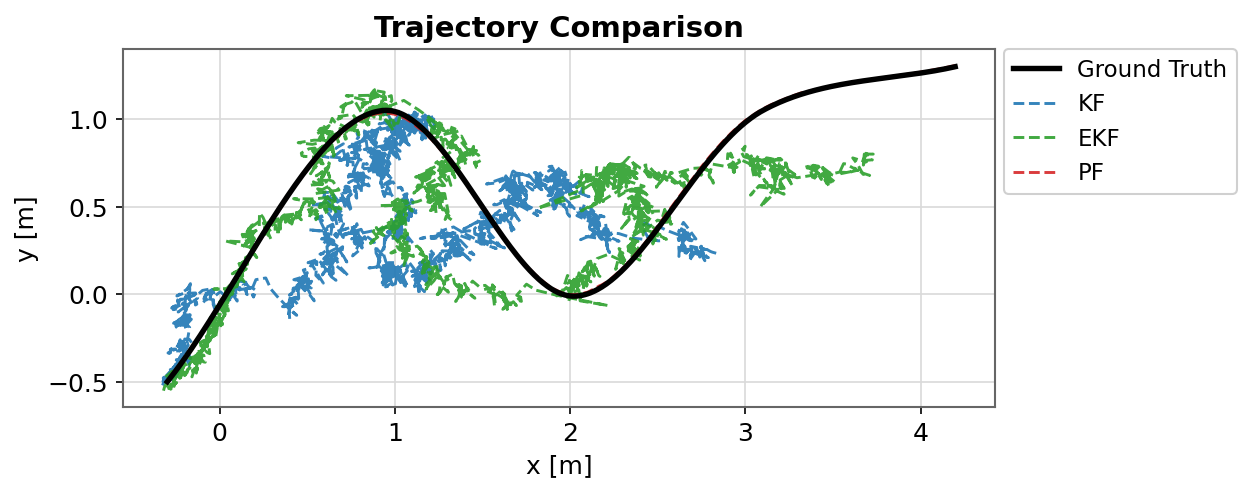
\includegraphics[width=0.98\columnwidth]{images/trajectories.png}
  \caption{Trajectory comparison on the S-slalom: Ground Truth (black),
           KF (blue dashed), EKF (green dashed), and PF (red dashed, tracking
           tightly under the ground-truth line).}
  \label{fig:traj}
\end{figure}

\subsection{Position Error and Accuracy}

Fig.~\ref{fig:poserr} shows the trajectory overlay together with the
position error over time for the three filters.
The PF error stays near a centimetre throughout, the EKF settles around a
tenth of a metre, and the KF error grows largest on the curved sections.
Table~\ref{tab:rmse} summarises the position and heading RMSE and the per-step
computational cost.
The PF is more than $20\times$ more expensive per step than the Gaussian
filters ($0.149$\,ms vs $\approx0.006$\,ms), yet it remains comfortably
real-time at 50\,Hz.

\begin{figure*}[!t]
  \centering
  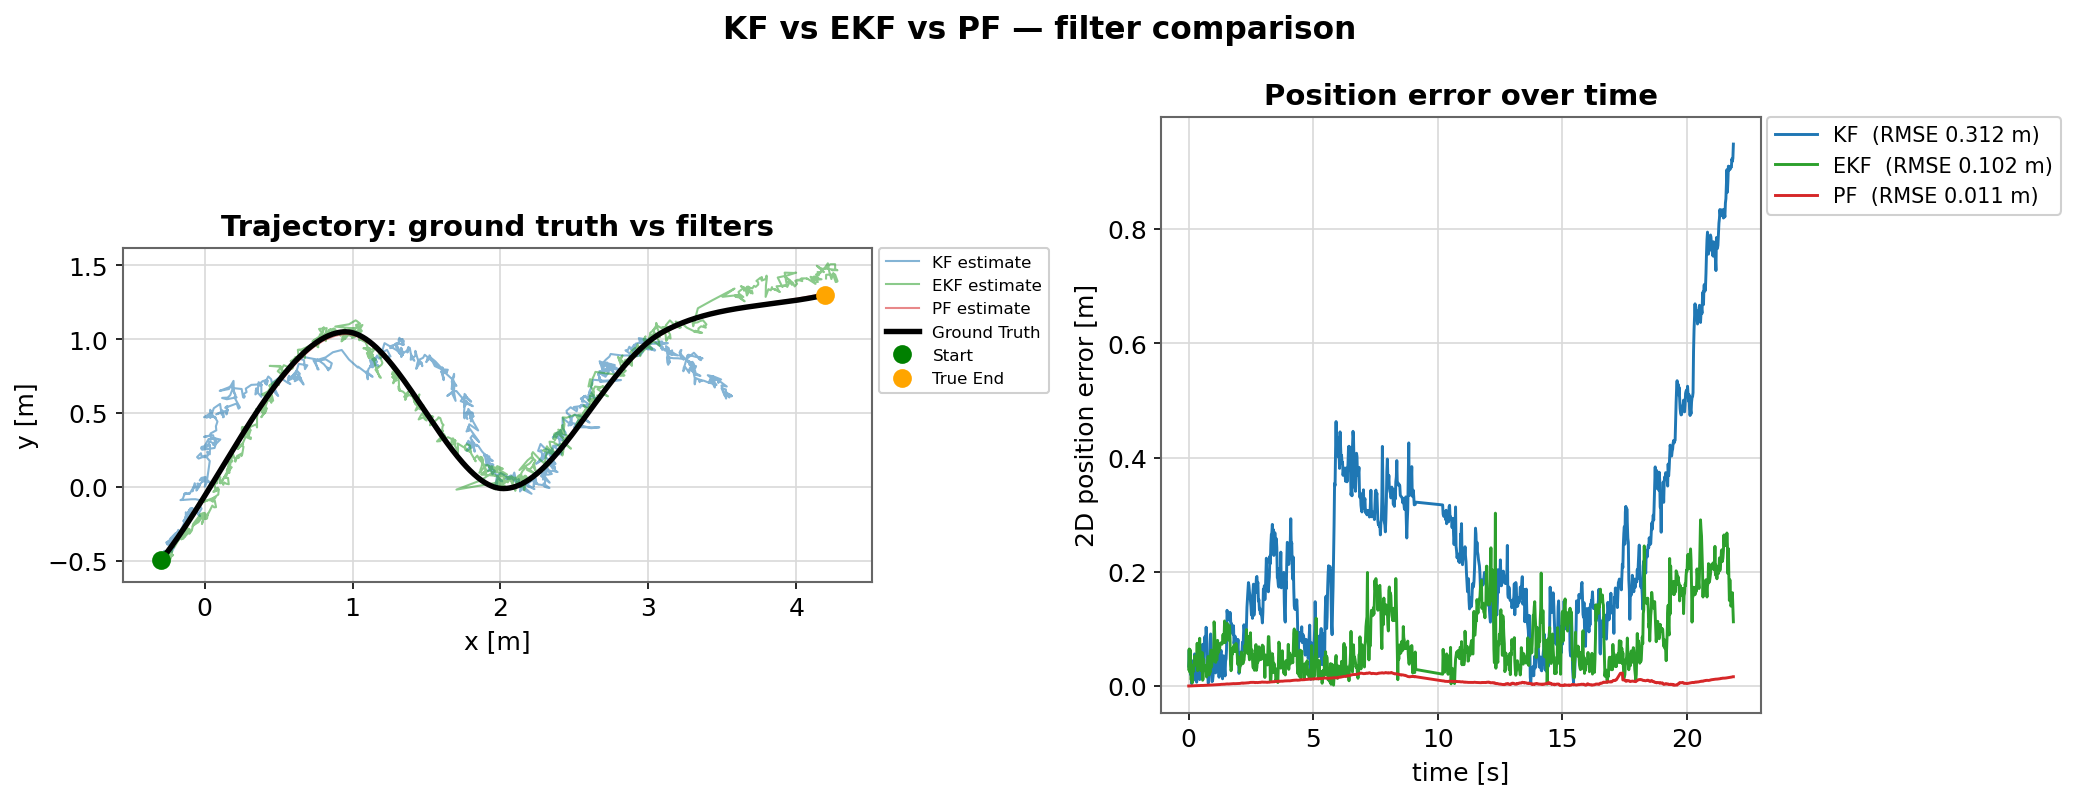
\includegraphics[width=0.95\textwidth]{images/position_error.png}
  \caption{Left: ground truth versus filter estimates. Right: 2-D position
           error over time for KF, EKF, and PF with RMSE annotations.}
  \label{fig:poserr}
\end{figure*}

\begin{table}[!h]
  \centering
  \setlength{\tabcolsep}{0.5em}
  {\renewcommand{\arraystretch}{1.2}
  \begin{tabular}{lccc}
    \toprule
    \textbf{Metric} & \textbf{KF} & \textbf{EKF} & \textbf{PF} \\
    \midrule
    Position RMSE [m]      & 0.312 & 0.102 & \textbf{0.011} \\
    Heading RMSE [$^\circ$]& 7.0   & 2.7   & \textbf{1.0}   \\
    Runtime / step [ms]    & 0.0054 & 0.0068 & 0.149 \\
    \bottomrule
  \end{tabular}}
  \caption{Baseline accuracy and runtime on the S-slalom trajectory.}
  \label{tab:rmse}
\end{table}

\subsection{Runtime and Complexity}

Fig.~\ref{fig:runtime} reports the measured per-update wall-clock cost together
with each filter's asymptotic complexity. The Gaussian filters cost
$\approx5$--$7\,\mu$s per step: their work is dominated by the $d\times d$
covariance products and the $m\times m$ gain inversion, i.e.\ $O(d^3)$ with state
dimension $d{=}3$ and measurement dimension $m{=}2$. The PF touches all $M{=}500$
particles in prediction, weighting and resampling, giving $O(M\,d)$ and a measured
$\approx149\,\mu$s --- about $25\times$ the EKF --- yet still two orders of
magnitude below the $20$\,ms budget at 50\,Hz.

\begin{figure}[!h]
  \centering
  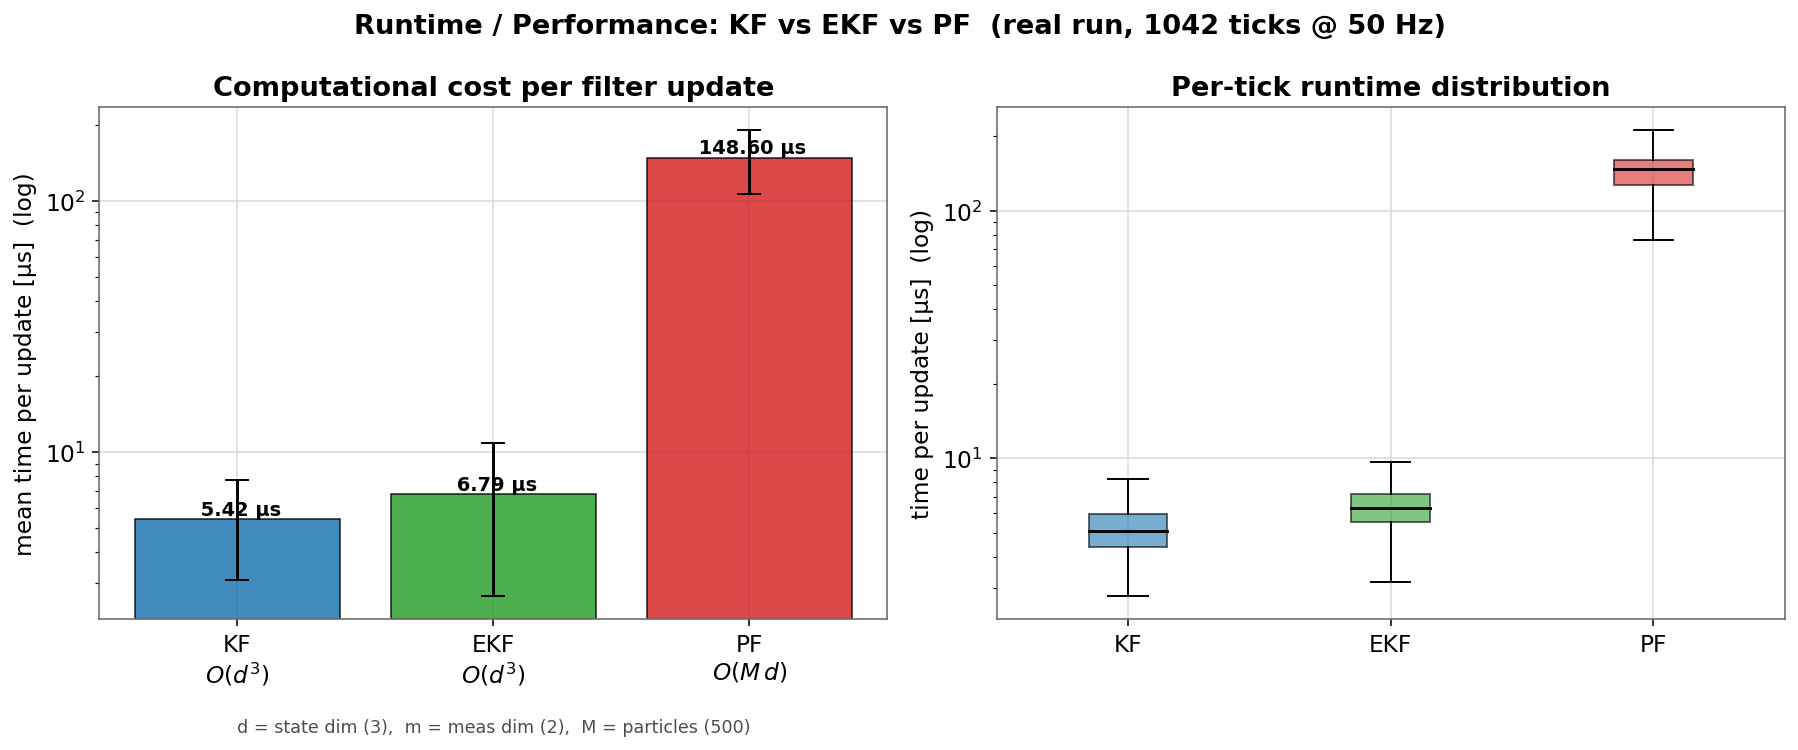
\includegraphics[width=0.98\columnwidth]{images/runtime_comparison.png}
  \caption{Measured per-update runtime (mean bar with std whiskers, log scale;
           right: per-tick distribution) annotated with the per-update asymptotic
           complexity. $d$ = state dim (3), $m$ = measurement dim (2),
           $M$ = particles (500).}
  \label{fig:runtime}
\end{figure}

\subsection{EKF Localization Analysis}

Fig.~\ref{fig:ekfloc} decomposes the localization process into three panels.
The left panel shows pure dead-reckoning that drifts away from ground truth
without corrections.
The centre panel adds the growing covariance circles, whose radius expands with
travelled distance.
The right panel shows the EKF output: with periodic landmark updates the
estimate snaps back onto the true track and the covariance stays bounded.
The odometry ends $0.90$\,m from the true end, whereas the landmark-corrected
EKF ends only $0.23$\,m away.

\begin{figure*}[!t]
  \centering
  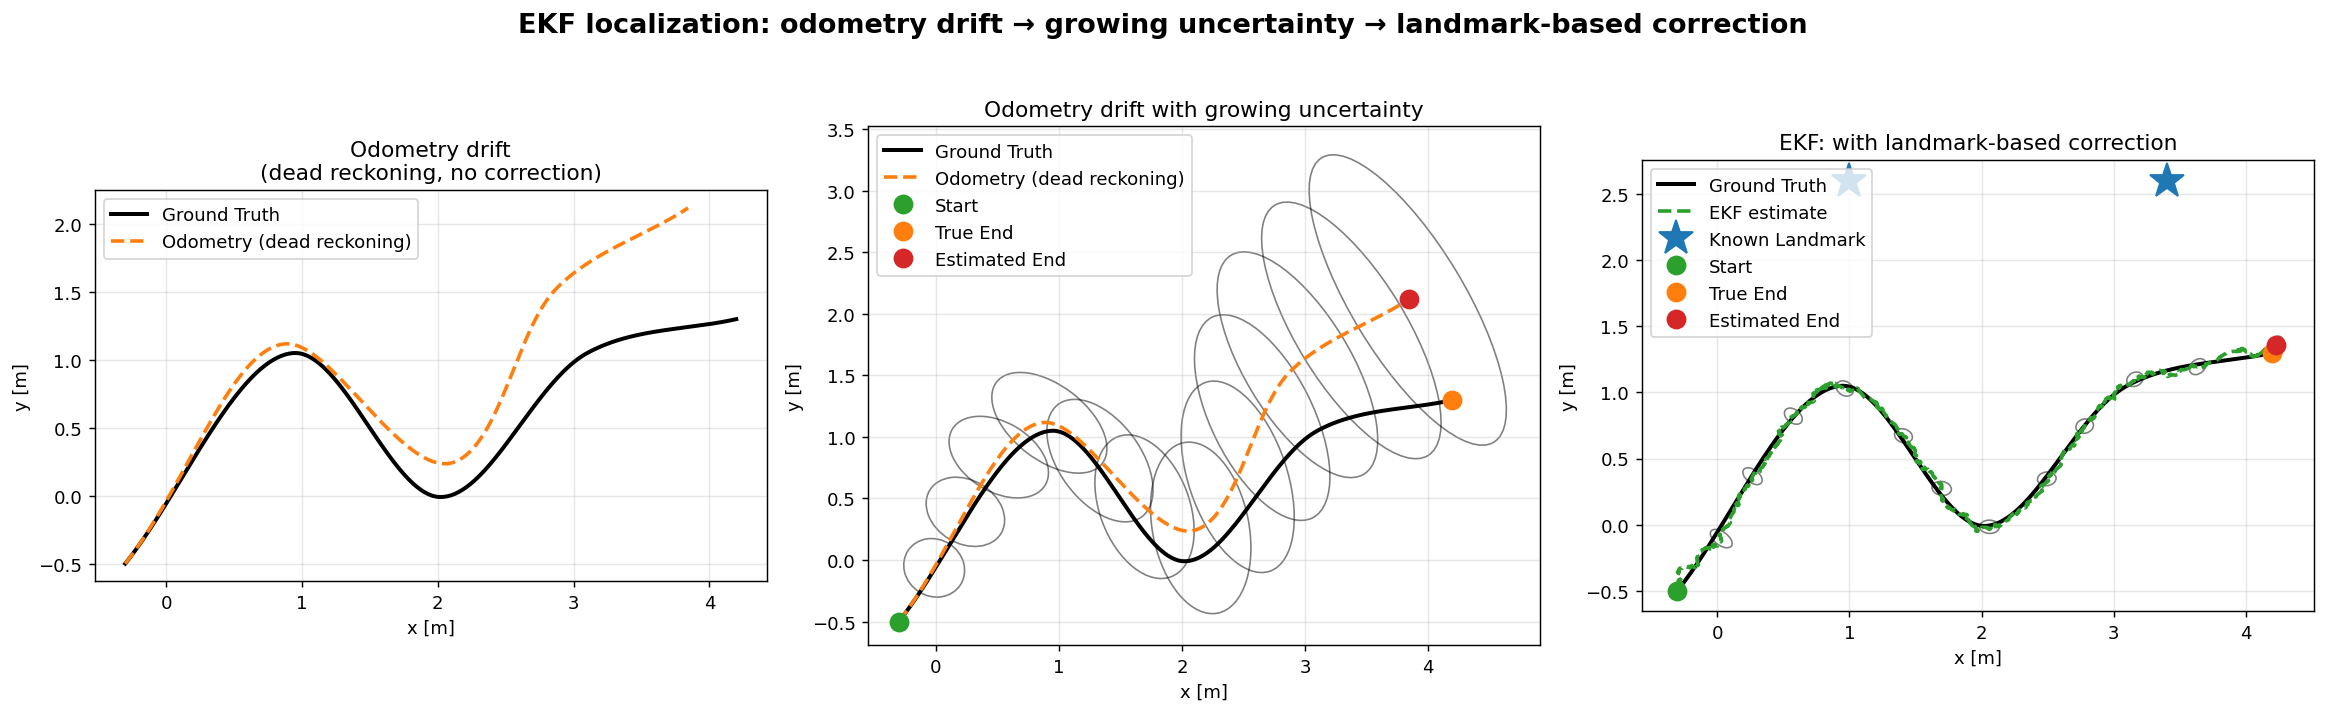
\includegraphics[width=0.95\textwidth]{images/ekf_localization.png}
  \caption{EKF localization on the S-slalom. Left: odometry drift without
           corrections. Centre: growing uncertainty (dead-reckoning only).
           Right: EKF estimate with landmark-based correction; the known
           landmark (star) keeps the estimate on the true path.}
  \label{fig:ekfloc}
\end{figure*}

\subsection{Effect of Measurement Delay}

Fig.~\ref{fig:delay} and Table~\ref{tab:delay} show the effect of artificial
measurement delay, while Fig.~\ref{fig:delaytraj} shows the EKF estimate on the
slalom at each delay level.
RMSE increases monotonically with delay for every filter, because a delayed
correction no longer aligns with the current robot position
\cite{Bar-Shalom2001Estimation}.
The PF is the most accurate at zero delay but degrades the most in relative
terms, since its tight estimate is the most penalised by the processing lag.

\begin{figure}[!h]
  \centering
  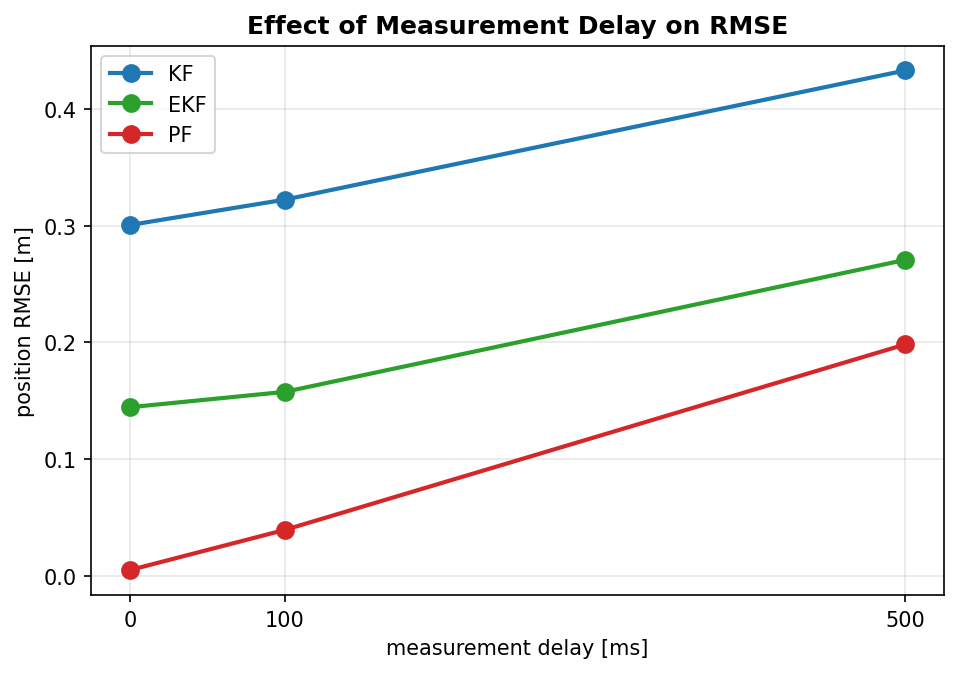
\includegraphics[width=0.92\columnwidth]{images/delay_comparison.png}
  \caption{Position RMSE versus measurement-processing delay for KF, EKF and PF.
           All filters degrade monotonically with delay.}
  \label{fig:delay}
\end{figure}

\begin{table}[!h]
  \centering
  \setlength{\tabcolsep}{0.5em}
  {\renewcommand{\arraystretch}{1.2}
  \begin{tabular}{lccc}
    \toprule
    \textbf{Delay} & \textbf{KF [m]} & \textbf{EKF [m]} & \textbf{PF [m]} \\
    \midrule
    0\,ms   & 0.301 & 0.145 & 0.005 \\
    100\,ms & 0.322 & 0.158 & 0.039 \\
    500\,ms & 0.433 & 0.271 & 0.198 \\
    \bottomrule
  \end{tabular}}
  \caption{Position RMSE under increasing measurement delay.}
  \label{tab:delay}
\end{table}

\begin{figure*}[!t]
  \centering
  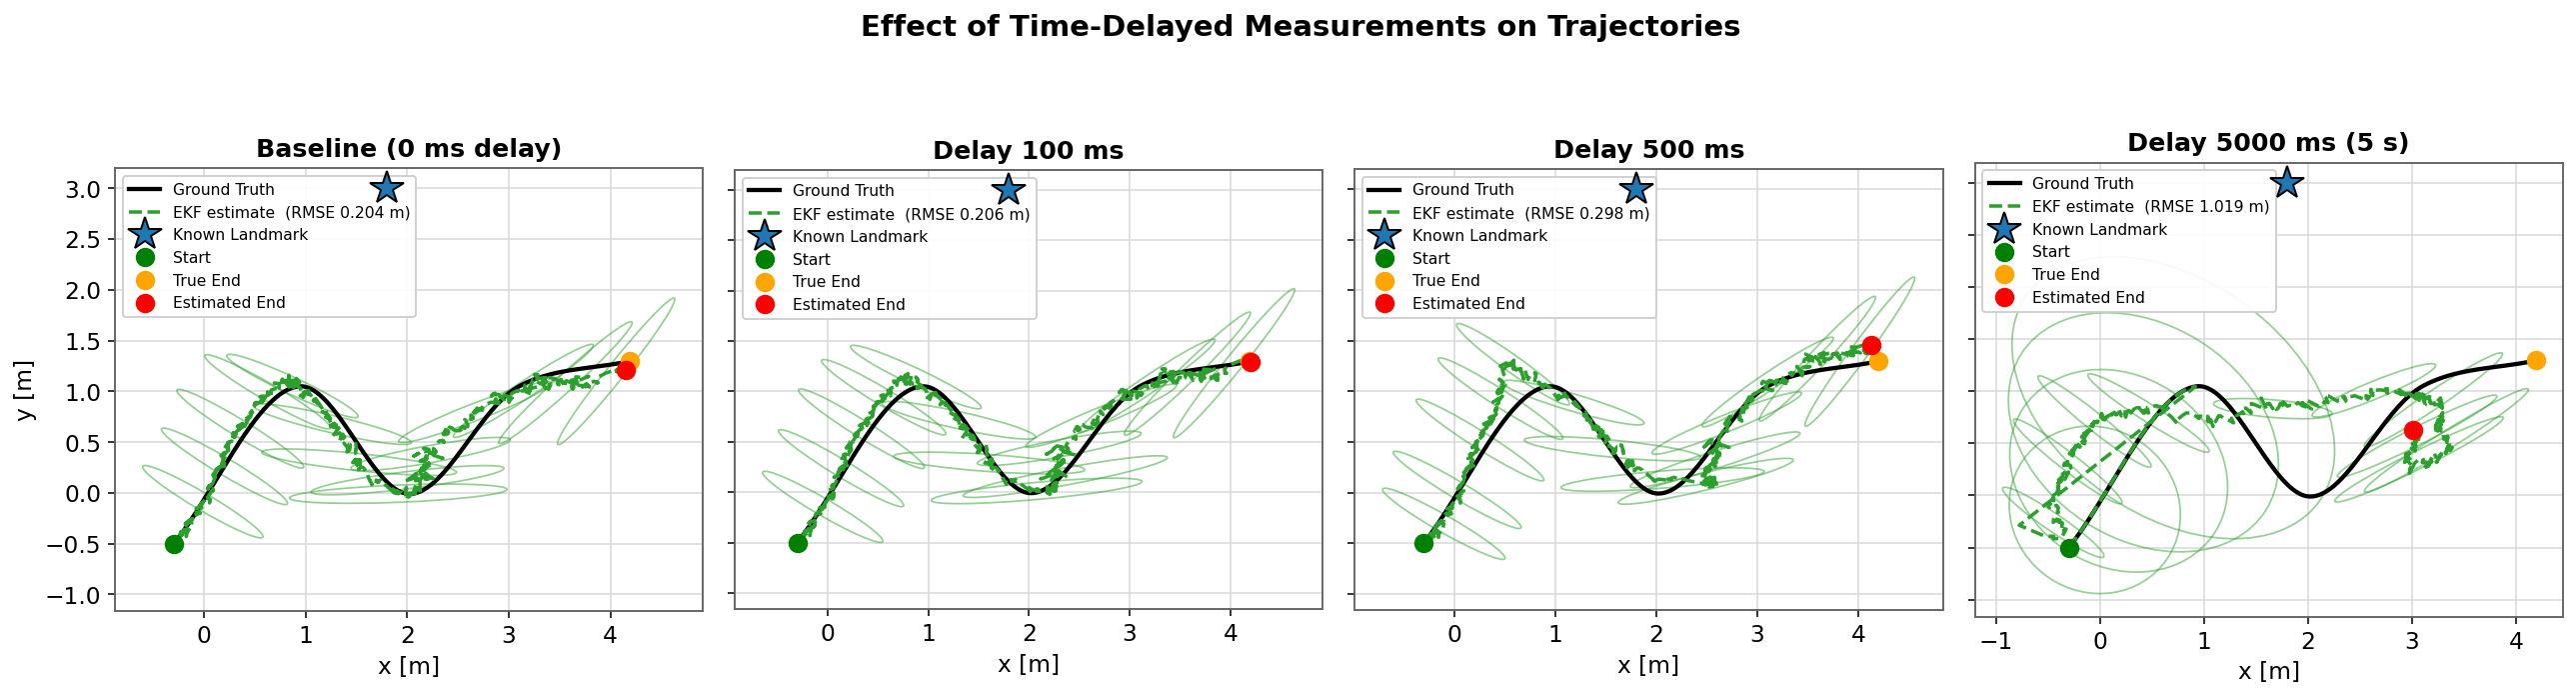
\includegraphics[width=0.98\textwidth]{images/delay_trajectories.png}
  \caption{EKF estimate on the S-slalom under increasing measurement-processing
           delay (0, 100, 500 and 5000\,ms): Ground Truth (black), EKF estimate
           (green dashed) with 2$\sigma$ covariance ellipses, and the known
           landmark (blue star). RMSE (averaged over 30 noise realisations) grows
           with delay; at 5\,s the stale correction no longer matches the current
           pose and the estimate diverges from the track (RMSE $\approx1.0$\,m).}
  \label{fig:delaytraj}
\end{figure*}

To locate each filter's tolerance limit we swept the delay from $0$ to
$5000$\,ms (Fig.~\ref{fig:breakdown}). With a $0.5$\,m usability threshold the KF
breaks almost immediately ($\approx250$\,ms), the EKF tolerates up to
$\approx1250$\,ms, and the PF stays usable beyond $5$\,s --- its RMSE merely
rises toward the open-loop dead-reckoning level rather than diverging. The
breaking delay scales inversely with speed, since the spatial lag is
$v\cdot\Delta t$.

\begin{figure}[!h]
  \centering
  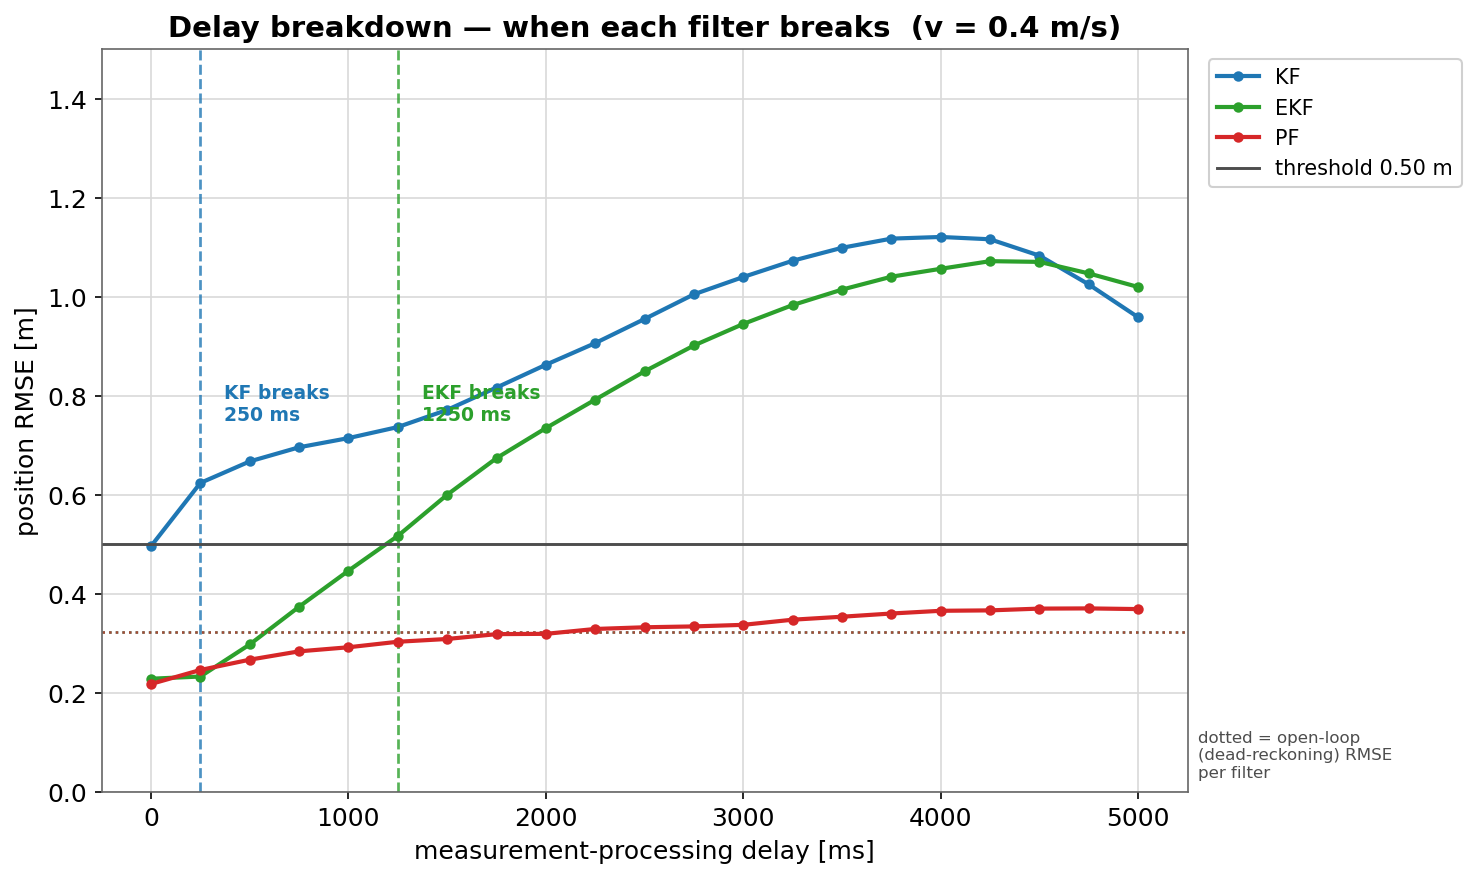
\includegraphics[width=0.98\columnwidth]{images/delay_breakdown.png}
  \caption{Delay breakdown: position RMSE versus measurement delay (12-seed mean)
           with each filter's breaking point (first delay with RMSE $>0.5$\,m).
           Dotted lines mark the open-loop (dead-reckoning) RMSE per filter.}
  \label{fig:breakdown}
\end{figure}

\subsection{Process-Noise (Q) and Measurement-Noise (R) Variation}

Fig.~\ref{fig:q} and Fig.~\ref{fig:r} report the $Q$ and $R$ sweeps for the EKF.
Both curves are U-shaped, confirming the existence of an optimum.
For the process noise, an optimum near $q_{xy}\!\approx\!10^{-5}$ minimises RMSE
($0.149$\,m): a smaller $Q$ makes the filter over-confident in its biased motion
model and it drifts, while a larger $Q$ makes it chase the noisy measurements and
become jittery.
For the measurement noise, the optimum is near $r\!\approx\!0.05$
($0.151$\,m): a smaller $R$ over-trusts the noisy sensor (jitter), while a larger
$R$ ignores the sensor and relies on the drifting model.
Together these experiments illustrate the model-confidence versus sensor-trust
trade-off encoded by $Q$ and $R$.

\begin{figure}[!h]
  \centering
  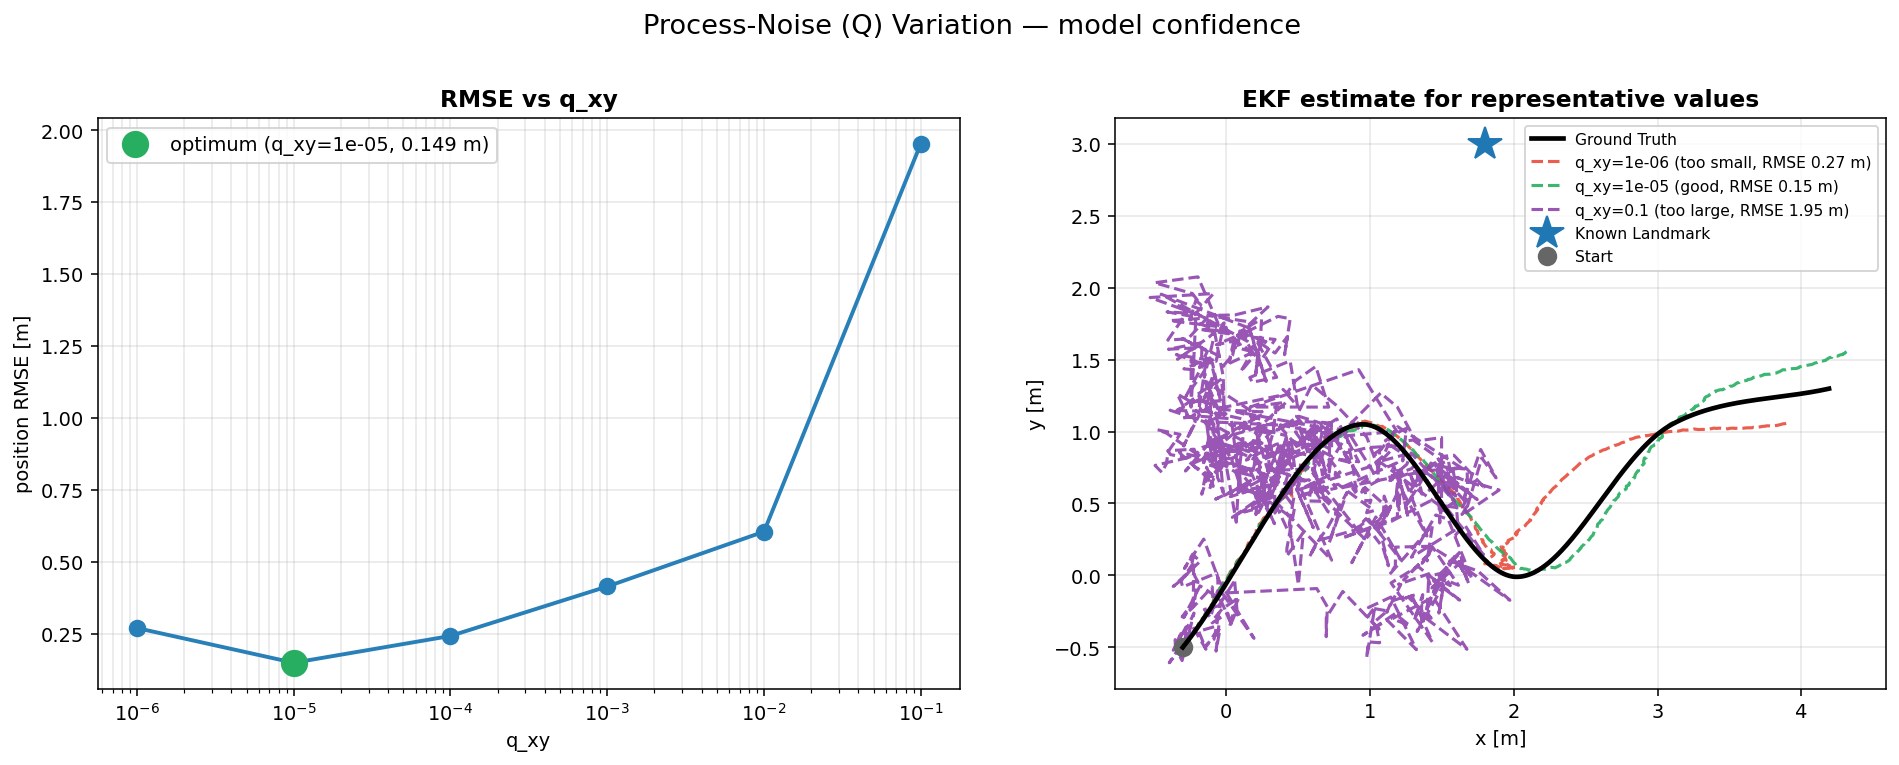
\includegraphics[width=0.98\columnwidth]{images/q_variation.png}
  \caption{Process-noise ($Q$) variation. Left: RMSE versus $q_{xy}$ with the
           optimum marked. Right: EKF estimate for representative values
           (too small, good, too large).}
  \label{fig:q}
\end{figure}

\begin{figure}[!h]
  \centering
  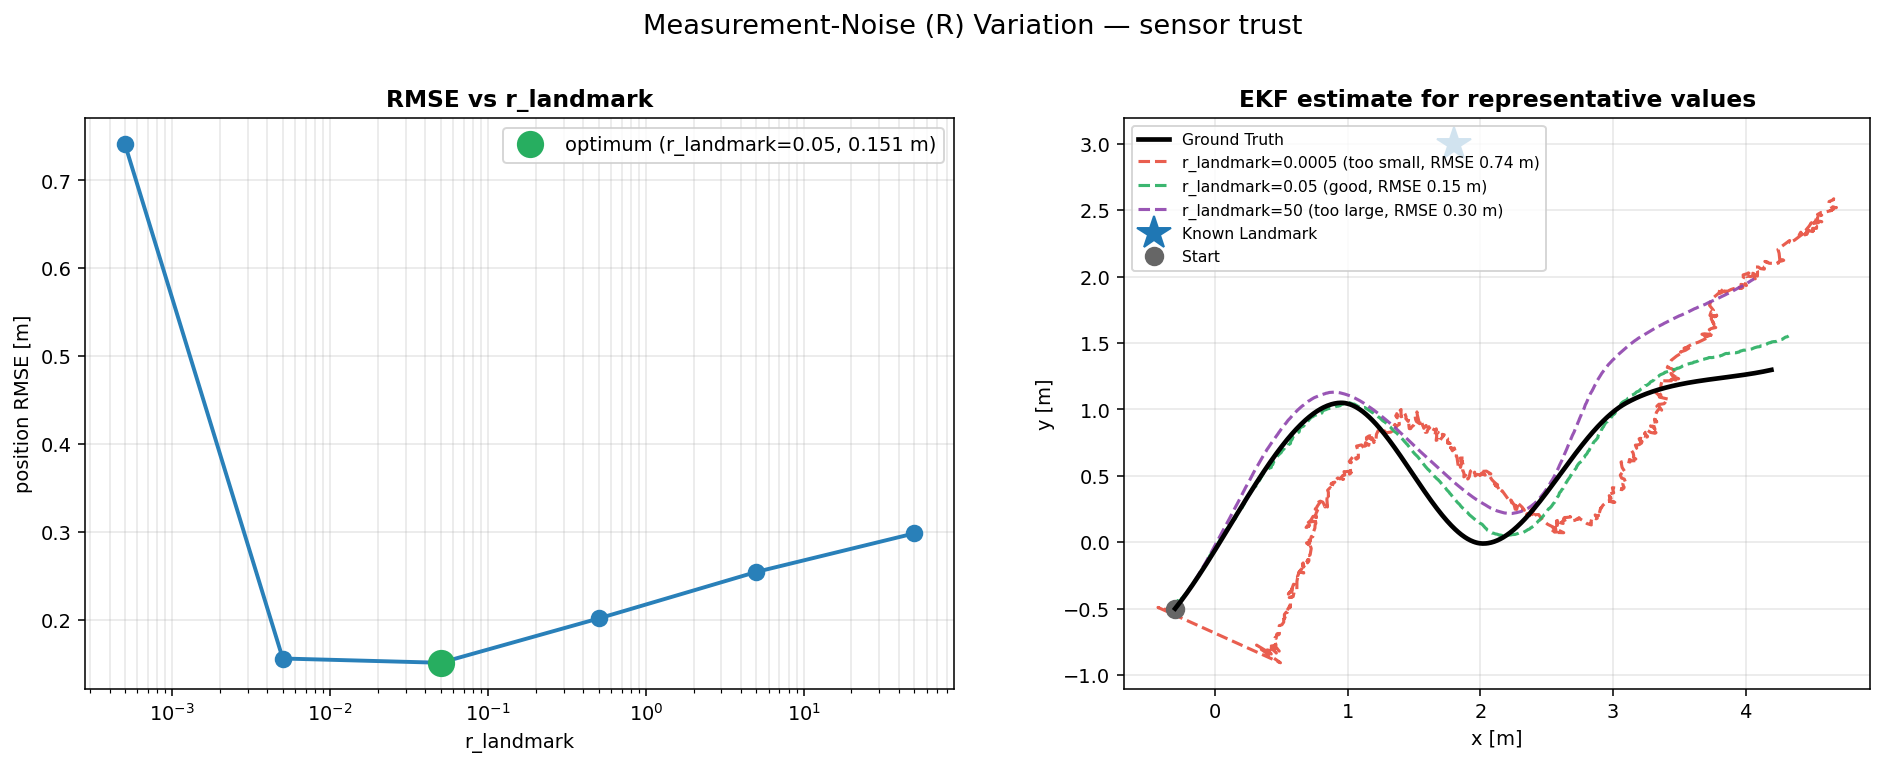
\includegraphics[width=0.98\columnwidth]{images/r_variation.png}
  \caption{Measurement-noise ($R$) variation. Left: RMSE versus $r$ with the
           optimum marked. Right: EKF estimate for representative values.}
  \label{fig:r}
\end{figure}

\subsection{Convergence from a Wrong Initial Pose}

To probe robustness we initialise each filter with a $1.0$\,m position error and
measure how the error decays (Fig.~\ref{fig:conv}). All three recover below
$0.5$\,m within $\approx0.02$\,s once the landmark is in view, but their
long-term behaviour differs sharply: the PF settles at $\approx0.16$\,m and
stays there, the EKF holds around $0.3$--$0.5$\,m, while the KF recovers briefly
and then drifts back up to $\approx1$\,m. The $F{=}I$ approximation makes the KF
over-confident after the first updates, so its gain becomes too small to track
the bias-driven drift --- the same mechanism that gives it the worst RMSE
overall.

\begin{figure}[!h]
  \centering
  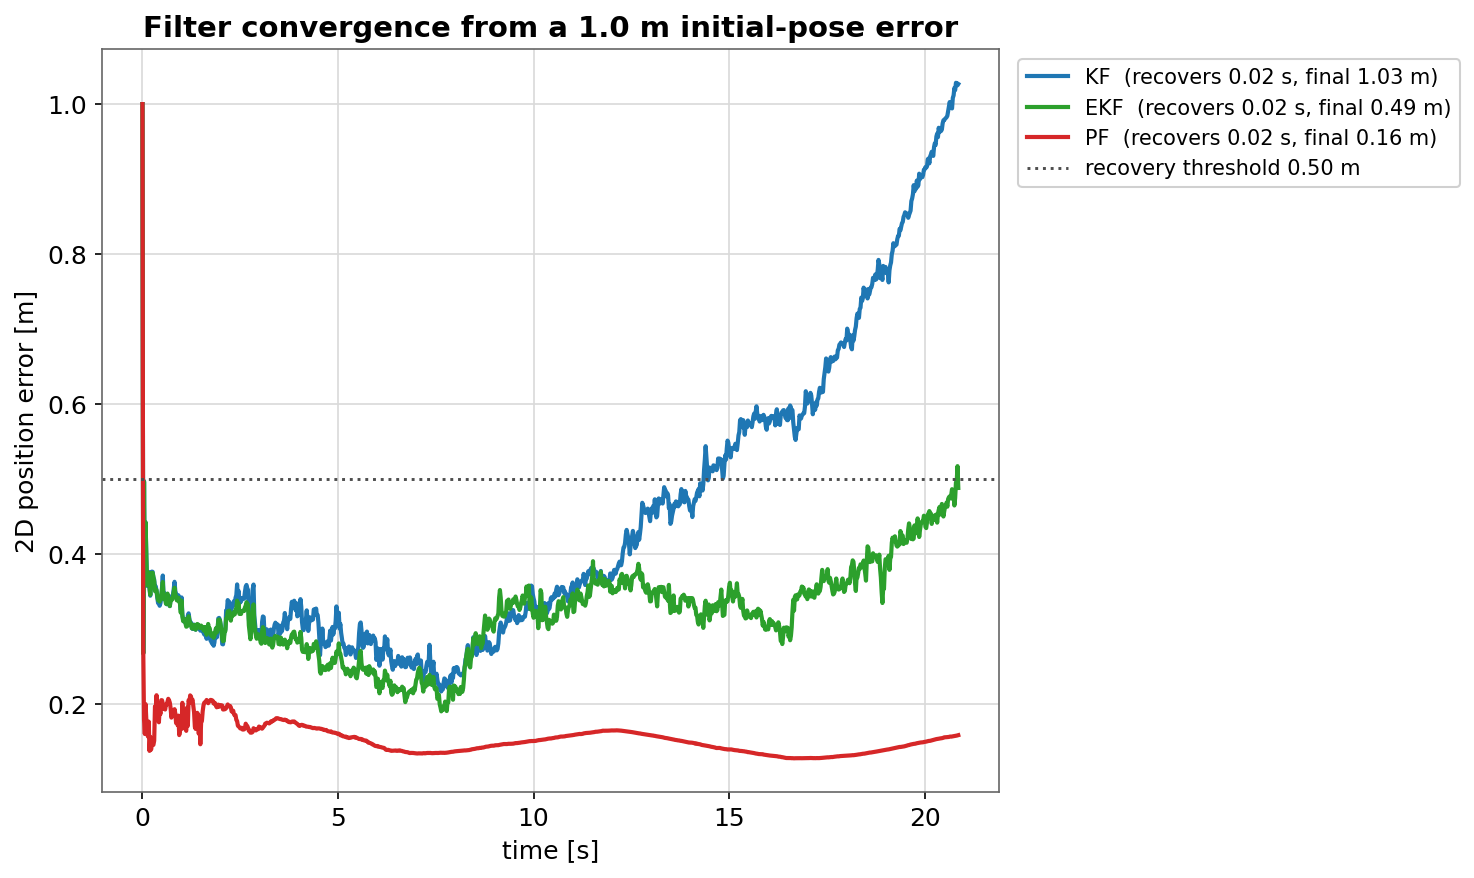
\includegraphics[width=0.98\columnwidth]{images/convergence.png}
  \caption{Convergence from a $1.0$\,m initial-pose error (12-seed mean position
           error over time). The PF recovers and stays low; the EKF holds; the KF
           recovers then destabilises.}
  \label{fig:conv}
\end{figure}

%%%%%%%%%%%%%%%%%%%%%%%%%%%%%%%%%%%%%%%%%%%%%%%%%%%%%%%%%%%%%%%%%%
\section{Summary and Outlook}
\label{sec:summary}

This paper compared KF, EKF, and PF for unicycle robot localization with a known
landmark, on an obstacle-avoiding S-slalom trajectory implemented in ROS\,2.
The PF achieved the lowest RMSE ($0.011$\,m), followed by the EKF
($0.102$\,m) and the KF ($0.312$\,m); the gap between KF and EKF is explained by
the EKF correctly propagating heading uncertainty into position via the motion
Jacobian, which the KF omits.
Measurement delays of up to $500$\,ms degraded all filters monotonically, the PF
being most sensitive, and the $Q$/$R$ sweeps revealed clear U-shaped optima that
quantify the model-confidence versus sensor-trust trade-off.
The study also surfaced and resolved several practical issues --- an
initial-pose launch bug, an unbounded trajectory, an EKF linearisation failure
near the landmark, and the non-reproducibility of best-effort real-time runs.

Future work should investigate: (1) multiple landmarks and ESS-gated resampling
to further improve PF robustness; (2) a 6-DOF model with full IMU pre-integration
for 3D environments; and (3) adaptive particle counts to balance accuracy and
computational cost.

%%%%%%%%%%%%%%%%%%%%%%%%%%%%%%%%%%%%%%%%%%%%%%%%%%%%%%%%%%%%%%%%%%
{\small
\bibliographystyle{IEEEtranS}
\bibliography{IEEEabrv,refs}
}

\clearpage
\section*{Appendix}

The complete set of plots and the scripts that generate them are provided in the
repository under \texttt{prol\_filters/scripts} and \texttt{data/}.
Fig.~\ref{fig:rmsebar} shows the baseline RMSE as a bar chart for quick reference.

\begin{figure}[!h]
  \centering
  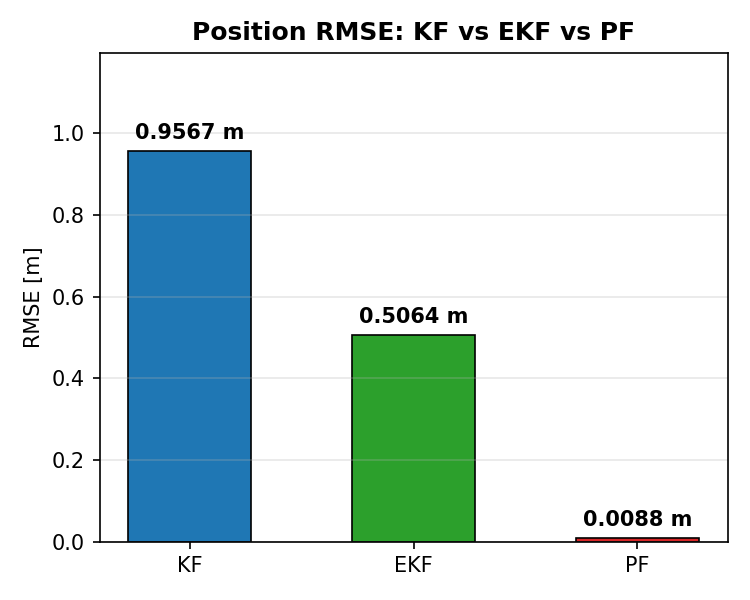
\includegraphics[width=0.75\columnwidth]{images/rmse_bar.png}
  \caption{Baseline position RMSE for KF, EKF and PF on the S-slalom.}
  \label{fig:rmsebar}
\end{figure}

\end{document}
